%\documentclass[doc,11pt]{apa6}
\documentclass[man,11pt]{apa6}
%\documentclass[jou,11pt]{apa6}
\usepackage{apacite}
\usepackage{setspace}
\usepackage{subfigure}
\usepackage{url}
\newcommand{\bibnodot}[1]{}

% margins
\setlength{\textheight}{9true in}
\setlength{\textwidth}{6.25true in}
\setlength{\topmargin}{-.43true in}
\setlength{\headheight}{.17true in}
\setlength{\headsep}{.25true in}
\setlength{\footskip}{.42true in}
\setlength{\topskip}{12pt}
\setlength{\oddsidemargin}{0.1true in}

\title{Predicting Weeding Decisions: Results}
\shorttitle{Predicting Weeding Decisions: Results}

\author{Kiri L. Wagstaff}
\affiliation{San Jose State University}
\note{\today}

\begin{document}
\maketitle

\section{Data Set Description}

This data set was obtained from Diane Klare and Lori Strethers of
Wesleyan University in March, 2015.
%
It contains 94,174 items identified as weeding candidates during a
large-scale weeding project that took place from 2011 to 2014 at
Wesleyan under the direction of Pat Tully.  Each item is marked to
indicate whether it was withdrawn or kept as a result of the weeding
project.

The goal of this project is to assess whether automated machine
learning classifiers can be trained to successfully reproduce human
judgments about whether items should be withdrawn or kept.

\section{Data Preprocessing}

I used the data set to create the following representation of items:
\singlespacing
\begin{center}
\begin{tabular}{|l|p{4.5in}|}
\hline
 {\em age} & Number of years between Publication Year and 2014, when the
  data was collected (integer ranging from 25 to 402). \\
 {\em checkouts} & The data set reports the number of checkouts
  since 1996.  The data set only includes items with fewer than 2
  checkouts, so this value is either 0 or 1 for all items. \\
 {\em shelftime} & Number of days since the last checkout, or -1
  if no last checkout is known (integer ranging from 763 to 6792, or -1). \\
 {\em uslib} & Number of U.S. libraries with a copy of this item,
  based on OCLC holdings records (integer ranging from 31 to 7634). \\
 {\em peerlib} & Number of peer libraries with a copy of this item,
  based on OCLC holdings records (integer ranging from 2 to 3;
  selection criteria for the data set included presence in at least
  two peer libraries). \\
 {\em hathicopy} & Does a copyrighted digital version exist in the
 Hathi Trust?  (boolean)\\
 {\em hathipub} & Does a public domain digital version exist in the
 Hathi Trust?  (boolean)\\
 {\em facultykeep} & Number of Wesleyan faculty votes to keep the item
  (integer ranging from 0 to 15). \\
 {\em librariankeep} & Number of Wesleyan librarian votes to keep the
  item (integer ranging from 0 to 1). \\
\hline
 {\em decision} & ``Withdraw'' or ``Keep''. \\
\hline
\end{tabular}
\end{center}
\doublespacing

I encountered some oddities in the data set.  In consultation with
Lori Strethers, I applied the following data cleaning steps:
\begin{itemize}
\item One item (``Germany's stepchildren,'' by Solomon Liptzin) had a
  ``Publication year'' of 5704.  The correct value is 1944.  I updated it
  in the database.

\item Lori indicated that items that are marked as part of an
  ``enumeration'' (series) were handled separately with different
  criteria, so I excluded them from the data set.  This affected 8,141
  items. 

\item Some items had a ``Date of last checkout'' after 1996, but the
   ``Checkouts since 1996'' field was 0.  Lori identified two causes:
(1) ``Multi-volume sets assign last circ date to all items in the set,
  but the number of checkouts is only incremented for the item checked out.''
(2)  ``Standalone items were checked out but not returned, and the 
  number of checkouts is incremented only when the item is returned.''
For both kinds of cases, I set the number of checkouts to 1.  This
affected 1,052 items.

\item Some items had no value for ``Date of last checkout'', but the
  ``Checkouts since 1996'' field was 1.  Lori explained: ``For these
  you can assume that it was checked out between 1996 and 2003.
  (System migration in 2003: items that were still charged out had
  their checkout date migrated, but items that had been returned just
  had a counter incremented to indicate how many times they had
  circulated.)''
%
Because we cannot be confident about the last checkout date for these
items, I decided to omit them from the data set. This affected 18,346
items. 

\end{itemize}

\section{Data Analysis}

\begin{figure}
\centering
\subfigure[{\em age}: Full data set]{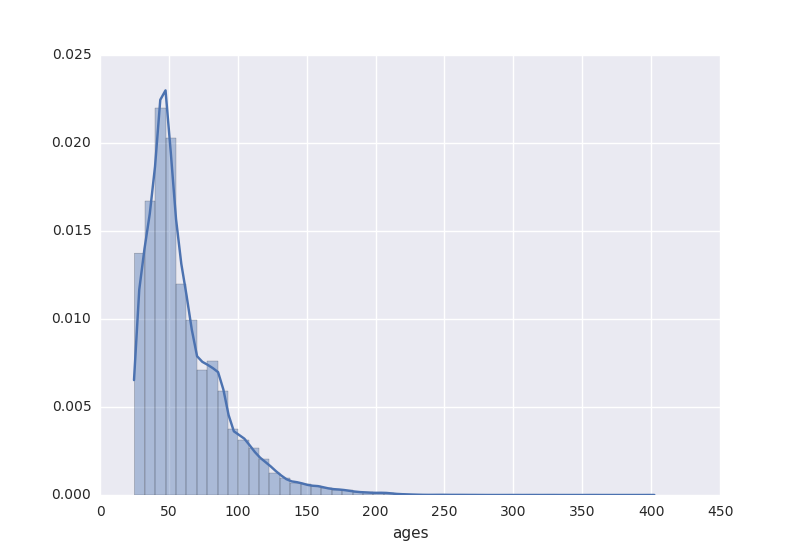
\includegraphics[width=3.1in]{../fig/hist-ages}} 
\subfigure[{\em age}: Split by decision]{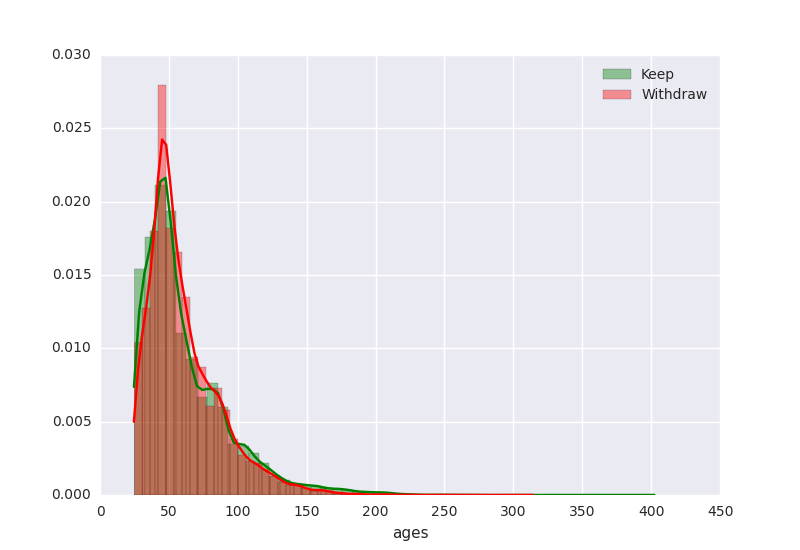
\includegraphics[width=3.1in]{../fig/hist-ages-split}}\\
\subfigure[{\em shelftime}: Full data set]{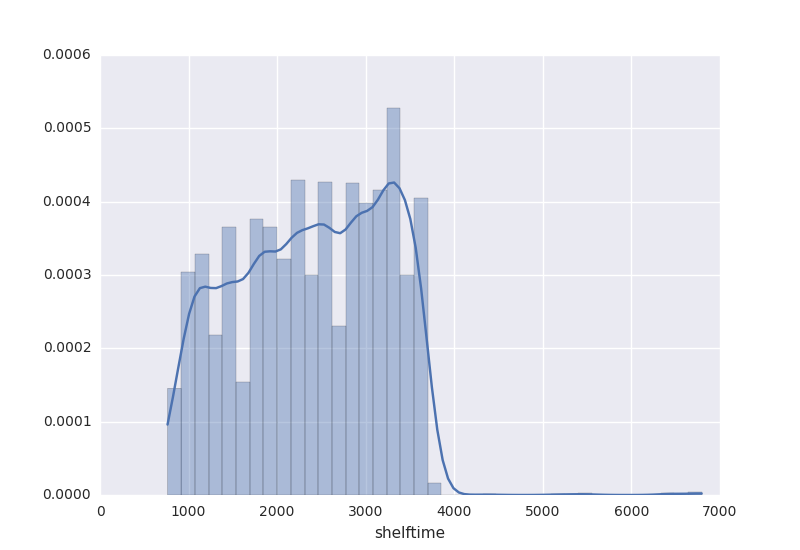
\includegraphics[width=3.1in]{../fig/hist-shelftime}} 
\subfigure[{\em shelftime}: Split by decision]{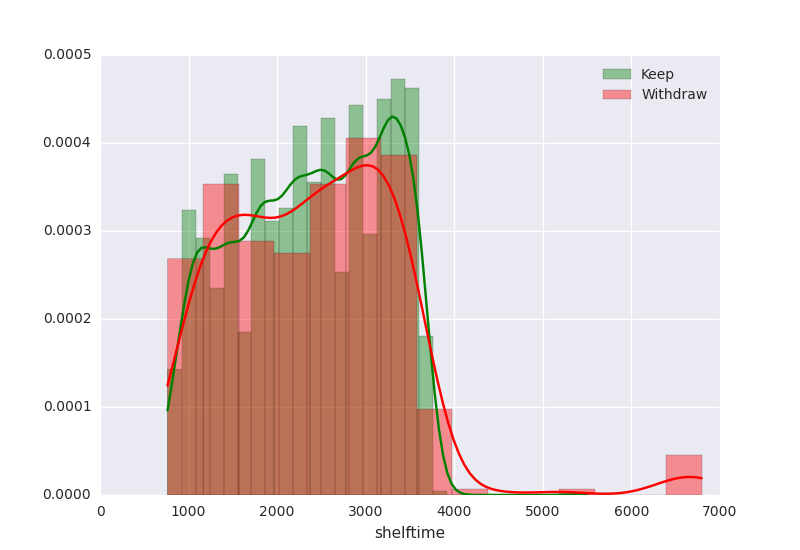
\includegraphics[width=3.1in]{../fig/hist-shelftime-split}}\\
\subfigure[{\em uslibs}: Full data set]{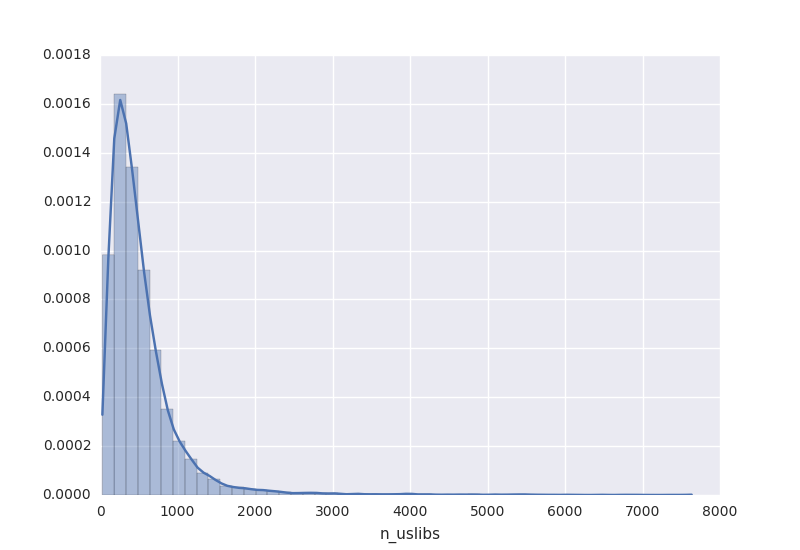
\includegraphics[width=3.1in]{../fig/hist-n_uslibs}}
\subfigure[{\em uslibs}: Split by
  decision]{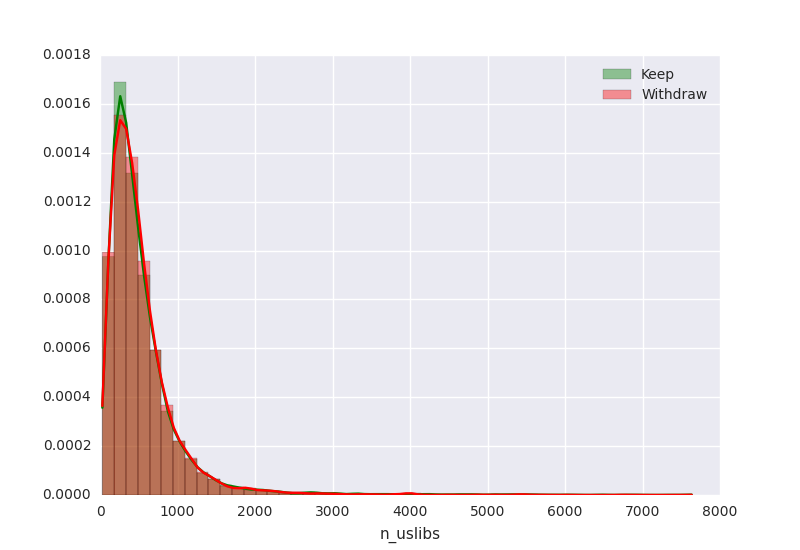
\includegraphics[width=3.1in]{../fig/hist-n_uslibs-split}}
\caption{Distribution of values observed for three variables (left
  column) as well as the distributions compiled separately for items
  marked ``Keep'' vs. ``Withdraw.''}
\label{fig:dist}
\end{figure}

The data set contains 67,687 items, 25,632 (38\%) of which are marked
``Withdraw'' and 42,055 (62\%) of which are marked ``Keep.''  

The minimum, mean, and maximum values for the four variables with more
than two distinct values are as follows:

\singlespacing
\begin{center}
\begin{tabular}{|l|ccc|}
\hline
Variable & Minimum & Mean & Maximum \\
\hline
 {\em age} & 25 & 61 & 402 \\
 {\em shelftime} & 763 & 2381 & 6792 \\
 {\em uslib} & 31 & 535 & 7634  \\
 {\em facultykeep} & 0 & 0 & 15 \\
\hline
\end{tabular}
\end{center}
\doublespacing

% Question: shelftime min is 763... was criteria that no checkout
% in last two years? I need to articulate their criteria above.

Figure~\ref{fig:dist} shows the distribution of values observed for
the first three variables (the fourth has very few non-zero values).
In general, we do not see a strong separation between ``Withdraw'' and
``Keep'' decisions for any single variable, except for {\em
  shelftime}, in which items with very large {\em shelftime} values
are more likely to be withdrawn, as we would expect.

For variables that take on only two possible values, I analyzed the
distribution of ``Keep'' adn ``Withdraw'' decisions.
%
The {\em checkouts} variable is dominated by items that have never
been checked out: 92\% of items in the data set have 0 checkouts.
The probability of an item being withdrawn, $P(W)$, given that it has
0 checkouts, is much higher than if it has 1 checkout (0.41 vs.~0.07).
The probability that an item is withdrawn, across the whole data set,
is 0.38. 

\singlespacing
\begin{center}
\begin{tabular}{|c|rr|rr|c|}
\hline
{\em checkouts} & Number & Fraction & Withdraw & Keep & $P(W)$\\ \hline
0 & 61,993 & 91.59\% & 25,252 & 36,741 & 0.41 \\
1 &  5,694 &  8.41\% &    380 &  5,314 & 0.07 \\
\hline
\end{tabular}
\end{center}
\doublespacing

The {\em peerlibs} variable is less strongly aligned with the weeding
decision, but there is still a difference between items that are held
by two peer libraries (60\% of the items, with $P(W) = 0.39$) versus
those held by three peer libraries (40\% of the items, with $P(W) =
0.36$).  The latter are less likely to be withdrawn.

\singlespacing
\begin{center}
\begin{tabular}{|c|rr|rr|c|}
\hline
{\em peerlibs} & Number & Fraction & Withdraw & Keep & $P(W)$\\ \hline
2 & 40,549 & 59.91\% & 15,991 & 24,558 & 0.39 \\
3 & 27,138 & 40.10\% &  9,641 & 17,497 & 0.36 \\
\hline
\end{tabular}
\end{center}
\doublespacing

Items in the Hathi Trust are more likely to be held in copyright
(56\%) than to be in the public domain (14\%).  For those items with a
copyrighted version in the Hathi Trust, the probability of being
withdrawn is higher (0.41) versus those items with a public domain
copy (0.37), which is very close to the data set average (0.38). 

\singlespacing
\begin{center}
\begin{tabular}{|c|rr|rr|c|}
\hline
{\em hathicopy} & Number & Fraction & Withdraw & Keep & $P(W)$\\ \hline
False & 29,518 & 43.61\% & 10,126 & 19,392 & 0.34 \\
True  & 38,169 & 56.39\% & 15,506 & 22,663 & 0.41 \\
\hline
\end{tabular}
\end{center}
\doublespacing

\singlespacing
\begin{center}
\begin{tabular}{|c|rr|rr|c|}
\hline
{\em hathipub} & Number & Fraction & Withdraw & Keep & $P(W)$\\ \hline
False & 58,149 & 85.91\% & 22,099 & 36,050 & 0.38 \\
True  &  9,538 & 14.10\% &  3,533 &  6,005 & 0.37 \\
\hline
\end{tabular}
\end{center}
\doublespacing

Finally, 13\% of the items have a value of 1 for the {\em
  librariankeep} variable.  There is a very strong relationship
between librarian votes and final decisions, as we expect: 98\% of
items with a ``Keep'' vote are kept (i.e.,~$P(W) = 0.02$).  The 211
items that were withdrawn despite a ``Keep'' vote were determined to
be either lost or duplicates of other items.

\singlespacing
\begin{center}
\begin{tabular}{|l|cc|cc|c|}
\hline
{\em librariankeep} & Number & Fraction & Withdraw & Keep & $P(W)$\\ \hline
0 & 58,754 & 86.80\% & 25,411 & 33,343 & 0.43 \\
1 &  8,933 & 13.20\% &    211 &  8,712 & 0.02 \\
\hline
\end{tabular}
\end{center}
\doublespacing


\section{Experimental Results}

I divided the data set randomly into two parts, one for training and
one for testing.  I evaluated several machine learning algorithms on
both data sets, after training.  I also evaluated baseline approaches
that predict ``Withdraw'' or ``Keep'' for all items.

To evaluate the agreement between the machine predictions and the
human decisions, I calculated the accuracy (fraction of predictions
that match human decisions) and the $\phi$ statistic (a measure of
agreement).  I also report the $p$-value at which the $\phi$ agreement
is considered to be statistically significant.

Given this definition of a contingency table:

\singlespacing
\begin{center}
\begin{tabular}{c|cc} 
 & \multicolumn{2}{c}{Human} \\
Classifier & Keep & Withdraw \\ \hline
Keep     & $a$ & $b$ \\ 
Withdraw & $c$ & $d$ \\ \hline
\end{tabular}
\end{center}
\doublespacing

The $\phi$ statistic is calculated as:

\begin{equation}
\phi = \frac{ad-bc}{\sqrt{(a+b)(c+d)(a+c)(b+d)}}
\end{equation}

Note that the baseline approach of predicting the same value for all
items will have either $a = b = 0$ or $c = d = 0$, so the $ad$ and
$bc$ terms in the numerator will be 0, and therefore $\phi$ is 0.

%Finally, to address the impact of classifier-assisted weeding on
%efficiency, a new statistic is defined.  The weeding efficiency
%advantage $E_W$ is defined as the ratio of the precision of the
%classifier's predictions to the precision of the human labels:
%\begin{equation}
%E_W = \frac{\frac{a}{a+b}}{\frac{a+c}{{a+b+c+d}}} =
%\frac{a(a+b+c+d)}{(a+b)(a+c)}
%\end{equation}
%This value quantifies the improvement that would be obtained by using
%the classifier's predictions to remove ``keep'' items from the
%candidate list.  

\singlespacing
\begin{center}
\begin{tabular}{|l|cc|cc|} \hline
Method & Training accuracy & Test accuracy & $\phi$ & Stat sig
\\ \hline
Baseline (all ``Withdraw'') & --- & 37.90\% & 0.00 & --- \\
Baseline (all ``Keep'') & --- & 62.10\% & 0.00 & --- \\ \hline
Decision tree          & 98.10\% & 69.11\% & 0.34 & $p=0.00$ \\
Random forest          & 96.33\% & 70.38\% & 0.37 & $p=0.00$ \\
3-nearest-neighbor     & 84.83\% & 70.92\% & 0.39 & $p=0.00$ \\
Naive Bayes            & 74.33\% & 74.41\% & 0.57 & $p=0.00$ \\
Support vector machine & 74.51\% & {\bf 74.65\%} & {\bf 0.58} & $p=0.00$ \\
% linear and RBF perform the same
\hline
\end{tabular}
\end{center}
\doublespacing

The support vector machine has the highest test accuracy and $\phi$
agreement statistic.  Several other classifiers suffer from
overfitting, in which the training accuracy is much higher than the
observed generalization performance on the test set.  All of the
$\phi$ values shown are statistically significant at the desired
$p=0.01$ level, i.e.,~we observe more agreement between classifier and
human judgments than would be expected at random.  However, a
better-than-random classifier may not be sufficiently reliable to be
of use in practice.

I also evaluated the classifier predictions obtained when using a
confidence threshold $\tau$ to restrict the classifier output to only
those items for which it has a posterior probability (confidence)
greather than $\tau$.  In this setting, the classifier might make
fewer predictions, but they are more likely to be reliable.

Figure~\ref{fig:res}(a) shows that accuracy increases as a function of
$\tau$ for all classifiers, but they increase at different rates.  A
single decision tree (DT) does not have a reliable method for
providing posterior probabilities, so varying $\tau$ has little
effect.  The other single classifier methods tend to provide posterior
probabilities that are clumped near zero or near a higher value,
yielding discontinuous jumps in performance.  The random forest (RF)
is an ensemble technique that incorporates voting from many individual
classifiers, so it yields a more continuous distribution of posterior
probabilities and a correspondingly smooth increase in accuracy as
$\tau$ increases.  

The support vector machine (SVM) classifier maintains the same
accuracy until $\tau$ reaches 0.7, at which point the classifier
generates predictions for only 13,088 items, and all of its predictions
are for ``Keep.''  Its selectivity is very reliable, yielding a high
accuracy (97.5\%) for this subset of items.  The SVM does not make any
predictions at $\tau=1.0$, so its results stop at $\tau=0.9$.
Similarly, the Naive Bayes (NB) classifier switches to all ``Keep''
decisions above a given $\tau$ value (1.0).

Figure~\ref{fig:res}(b) reports the $\phi$ (agreement) values observed
as $\tau$ is increased.  For most values of $\tau$, the SVM classifier
has the highest $\phi$ agreement with human labels, as was shown in
the initial table of results (the table corresponds to $\tau=0$).
However, for $\tau >= 0.7$, SVM agreement drops dramatically.  While
overall accuracy is high, this is largely due to correct ``Keep''
predictions, and $\phi$ penalizes lopsided performance.  For high
$\tau$ values, the 3-NN classifier yields higher agreement, and at
$\tau = 1.0$, RF has the highest agreement.  As noted above, $\phi$ is
$0.0$ if the predicted decisions all fall into one class or the other,
which occurs for the SVM and NB at $\tau=1.0$.

We can better understand the different classifier results by examining
what kinds of errors they make.  Figure~\ref{fig:res}(c) shows
classifier {\em recall}, which is the fraction of items labeled by
humans as ``Withdraw'' for which the classifier correctly predicted
``Withdraw.''  Again we see that the SVM and NB are very good at
correctly predicting ``Withdraw'' for a large fraction ($> 96$\%) of
the items that were truly withdrawn, until $\tau$ reaches 0.7 (SVM) or
1.0 (NB), at which point they only predict ``Keep''.  For most
classifiers, as $\tau$ increases, recall decreases, generally because
the total number of predictions made by the classifier declines.

The other side of the coin is {\em precision}, which is the fraction
of items predicted by the classifier as ``Withdraw'' that were
actually withdrawn.  Figure~\ref{fig:res}(d) shows that precision
tends to increase as $\tau$ increases, indicating that the more
confident decisions tend to more accurately predict item
withdrawal. No value is shown for the sVM or NB at $\tau$ values for
which they do not predict any ``Withdraw'' items.

% Plot of Test acc as a fn of confidence threshold
% Plot of Phi as a fn of confidence threshold
% Plot of recall and precision
\begin{figure}
\centering
\subfigure[Accuracy]{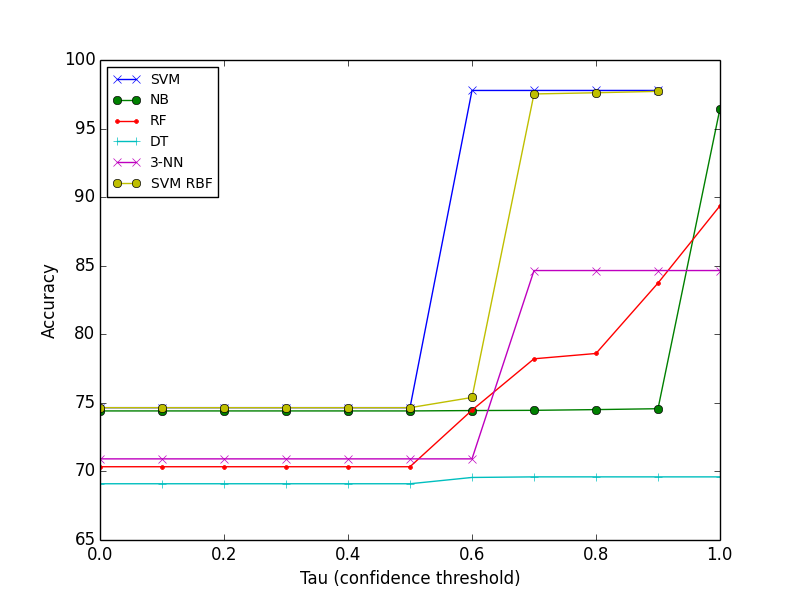
\includegraphics[width=3.1in]{../fig/tau-Accuracy}}
\subfigure[Phi]{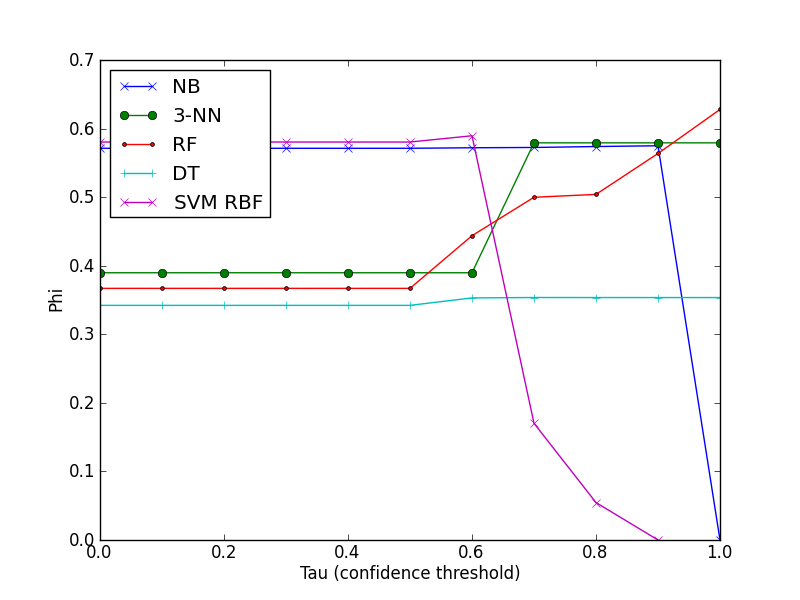
\includegraphics[width=3.1in]{../fig/tau-Phi}}
\subfigure[Recall]{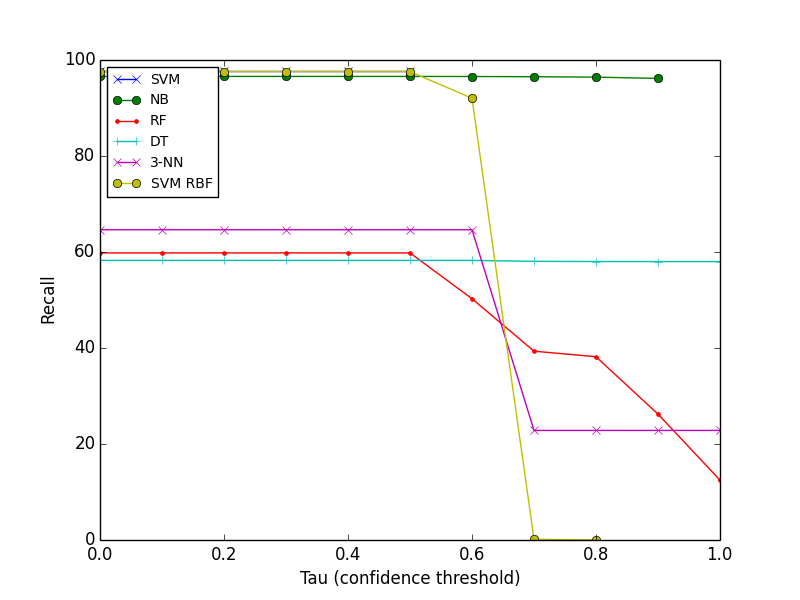
\includegraphics[width=3.1in]{../fig/tau-Recall}}
\subfigure[Precision]{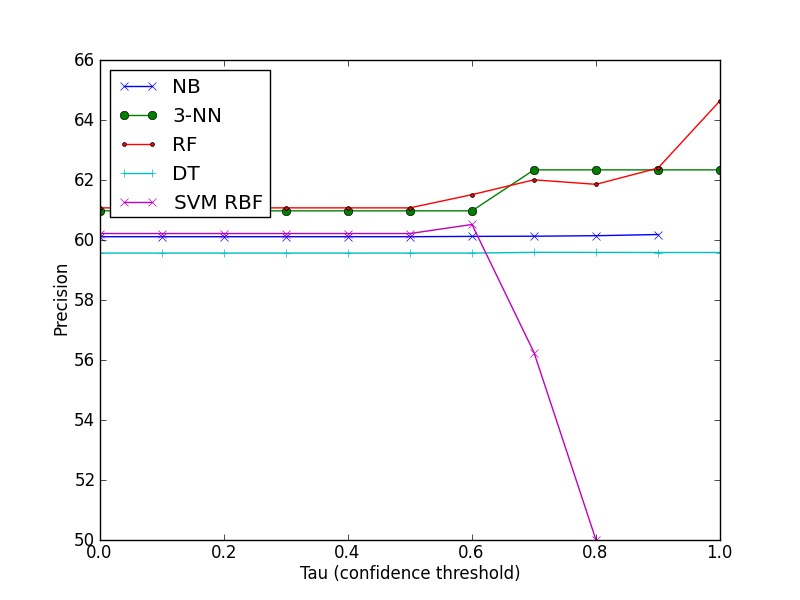
\includegraphics[width=3.1in]{../fig/tau-Precision}}
\caption{Classifier results in predicting weeding decisions when
  varying the confidence threshold, $\tau$.}
\label{fig:res}
\end{figure}

Finally, Figure~\ref{fig:eff} provides a different view of the
precision results in which the classifier precision is normalized by
the precision of the original full candidate list.  The {\em
  efficiency} of a classifier's output is this ratio, which captures
the degree to which using the classifier to filter the list of
candidates can reduce librarian review effort.  A value of 1.0 would
indicate that the classifier's precision is the same as the original
list's precision, and higher values are better.  The relative ordering
of the methods is the same as those seen in the precision plot.  We
observe that all classifiers can increase the efficiency of the
weeding process, with improvements ranging from 31-71\%.

\begin{figure}
\centering
% Plot of Weeding efficiency as a fn of confidence threshold
\subfigure[Efficiency]{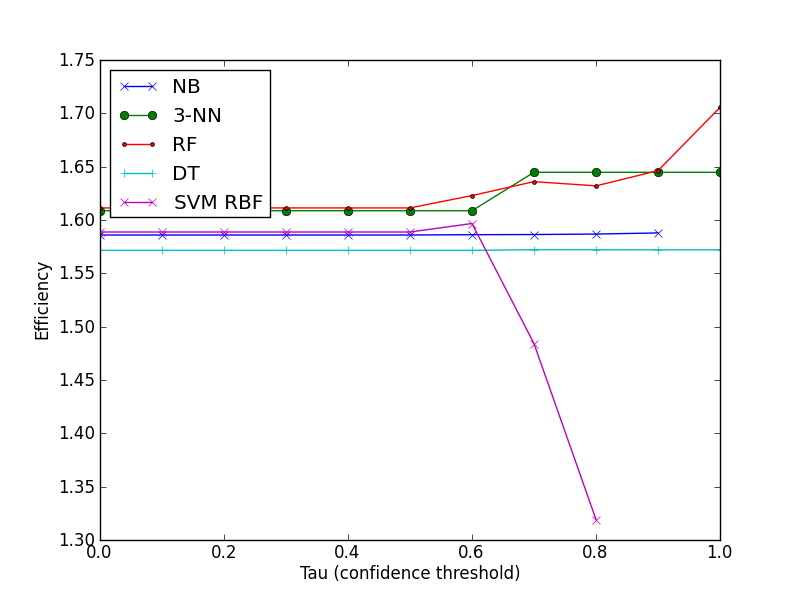
\includegraphics[width=3.1in]{../fig/tau-Efficiency}}
\caption{Classifier efficiency in predicting weeding decisions when
  varying the confidence threshold, $\tau$.}
\label{fig:eff}
\end{figure}

\section{Discussion of Results}

The level of agreement between machine and human weeding decisions
that was achieved using the current representation reached a maximum
of 0.58 (accuracy of 74.65\%), using a support vector machine.  While
this is statistically significant agreement, the large size of the
data set seems to render significant even low levels of agreement,
such as 0.34 (69.11\% accuracy) achieved by the decision tree.

All of the machine learning classifiers performed better than either
baseline approach in terms of accuracy.  This indicates that they
successfully leveraged information in the features.  However, they did
not out-perform the ``Keep'' baseline by a large margin.

We observe higher accuracy, $\phi$ agreement, and precision by
retaining only the most confident machine predictions, rather than
relying on the machine to make predictions for all items.  This is a
tradeoff; recall tends to go down as $\tau$ increases and the
classifier makes fewer predictions.

The examination of recall and precision, as a function of $\tau$,
provides useful guidance for selecting which classifier would be of
most use for a future weeding project.  If we wish to maximize the
efficiency of librarian time when reviewing items for possible
withdrawal, then we want precision to be as high as possible.  High
precision indicates that a large fraction of the candidates given to
the librarian to review will ultimately be withdrawn.  The best
precision, and highest $\phi$ agreement, are achieved by the random
forest (RF) classifier with a $\tau$ value of 1.0.  This yields a
classifier efficiency of 1.71, indicating that a librarian examining
the 14,321 items selected by the RF classifier (regardless of their
prediction) would find 71\% more genuine ``withdraw'' candidates than
spending the same time on the same number of items randomly pulled
from the initial candidate list.

\section{Notes}

As planned in my previous update, I added the confidence-based
evaluation of performance as a function of $\tau$, and I added the
Hathi Trust variables and omitted items with missing values.

However, I have been unsuccessful at doing a scripted lookup of items
in the dataset to see if they are contained in {\em Resources for
  College Libraries}.  The requirement of an SJSU login can be easily
met in a web browser, but I have not been able to get this to work
from the command line or a script, which is the only feasible way to
look up 67,000 items in a reasonable amount of time.  However, the
results currently obtained may be sufficiently interesting without the
inclusion of this variable.  I do not have any evidence that including
it would make a significant difference in the outcome.

\end{document}
